% Options for packages loaded elsewhere
\PassOptionsToPackage{unicode}{hyperref}
\PassOptionsToPackage{hyphens}{url}
%
\documentclass[
]{article}
\usepackage{amsmath,amssymb}
\usepackage{lmodern}
\usepackage{iftex}
\ifPDFTeX
  \usepackage[T1]{fontenc}
  \usepackage[utf8]{inputenc}
  \usepackage{textcomp} % provide euro and other symbols
\else % if luatex or xetex
  \usepackage{unicode-math}
  \defaultfontfeatures{Scale=MatchLowercase}
  \defaultfontfeatures[\rmfamily]{Ligatures=TeX,Scale=1}
\fi
% Use upquote if available, for straight quotes in verbatim environments
\IfFileExists{upquote.sty}{\usepackage{upquote}}{}
\IfFileExists{microtype.sty}{% use microtype if available
  \usepackage[]{microtype}
  \UseMicrotypeSet[protrusion]{basicmath} % disable protrusion for tt fonts
}{}
\makeatletter
\@ifundefined{KOMAClassName}{% if non-KOMA class
  \IfFileExists{parskip.sty}{%
    \usepackage{parskip}
  }{% else
    \setlength{\parindent}{0pt}
    \setlength{\parskip}{6pt plus 2pt minus 1pt}}
}{% if KOMA class
  \KOMAoptions{parskip=half}}
\makeatother
\usepackage{xcolor}
\usepackage[margin=1in]{geometry}
\usepackage{longtable,booktabs,array}
\usepackage{calc} % for calculating minipage widths
% Correct order of tables after \paragraph or \subparagraph
\usepackage{etoolbox}
\makeatletter
\patchcmd\longtable{\par}{\if@noskipsec\mbox{}\fi\par}{}{}
\makeatother
% Allow footnotes in longtable head/foot
\IfFileExists{footnotehyper.sty}{\usepackage{footnotehyper}}{\usepackage{footnote}}
\makesavenoteenv{longtable}
\usepackage{graphicx}
\makeatletter
\def\maxwidth{\ifdim\Gin@nat@width>\linewidth\linewidth\else\Gin@nat@width\fi}
\def\maxheight{\ifdim\Gin@nat@height>\textheight\textheight\else\Gin@nat@height\fi}
\makeatother
% Scale images if necessary, so that they will not overflow the page
% margins by default, and it is still possible to overwrite the defaults
% using explicit options in \includegraphics[width, height, ...]{}
\setkeys{Gin}{width=\maxwidth,height=\maxheight,keepaspectratio}
% Set default figure placement to htbp
\makeatletter
\def\fps@figure{htbp}
\makeatother
\setlength{\emergencystretch}{3em} % prevent overfull lines
\providecommand{\tightlist}{%
  \setlength{\itemsep}{0pt}\setlength{\parskip}{0pt}}
\setcounter{secnumdepth}{-\maxdimen} % remove section numbering
\ifLuaTeX
  \usepackage{selnolig}  % disable illegal ligatures
\fi
\IfFileExists{bookmark.sty}{\usepackage{bookmark}}{\usepackage{hyperref}}
\IfFileExists{xurl.sty}{\usepackage{xurl}}{} % add URL line breaks if available
\urlstyle{same} % disable monospaced font for URLs
\hypersetup{
  pdftitle={Overall Trends},
  hidelinks,
  pdfcreator={LaTeX via pandoc}}

\title{Overall Trends}
\author{}
\date{\vspace{-2.5em}}

\begin{document}
\maketitle

\hypertarget{overall-engagement}{%
\subsection{Overall Engagement}\label{overall-engagement}}

\begin{center}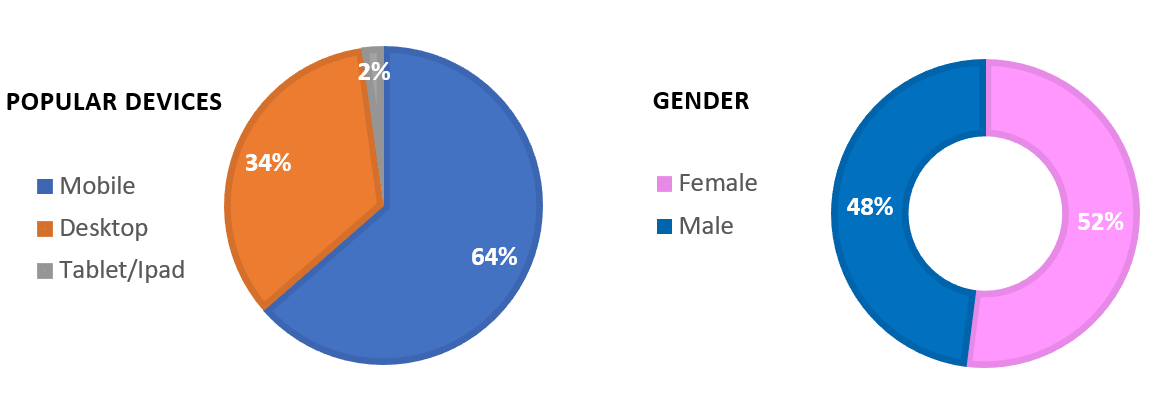
\includegraphics[width=0.9\linewidth,height=0.9\textheight]{/Users/leonardo.urbiola_fox/Desktop/R Studio/Audience/general_1} \end{center}

\begin{center}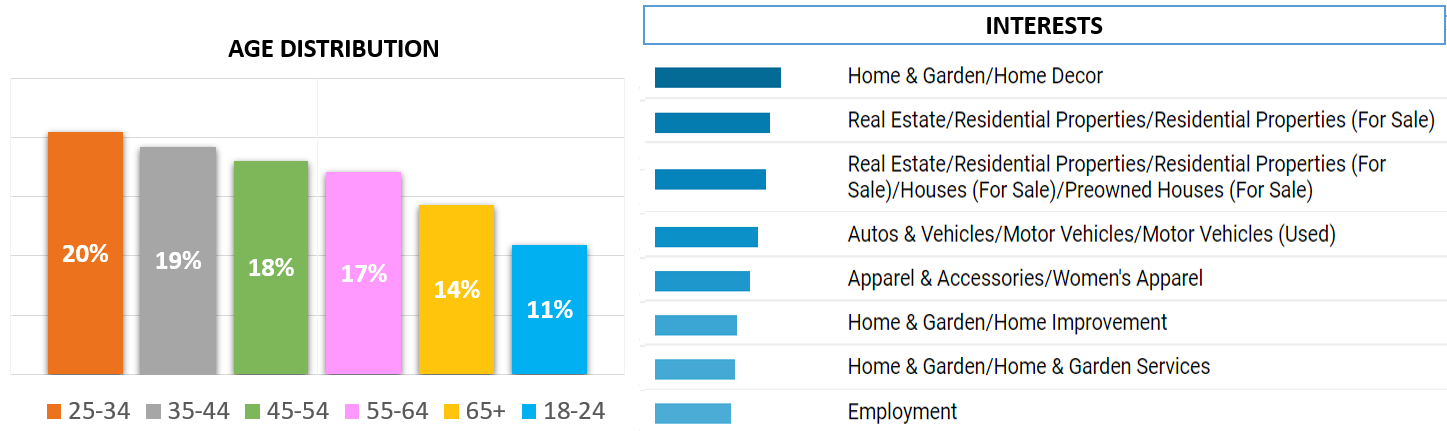
\includegraphics[width=1\linewidth,height=1\textheight]{/Users/leonardo.urbiola_fox/Desktop/R Studio/Audience/general_2} \end{center}

\begin{center}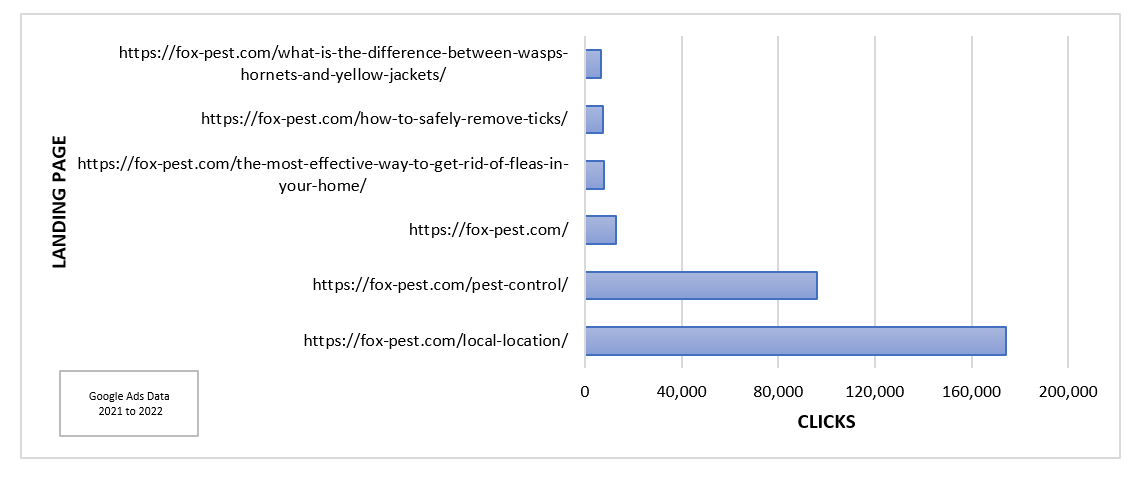
\includegraphics[width=1\linewidth,height=1\textheight]{/Users/leonardo.urbiola_fox/Desktop/R Studio/Audience/landing} \end{center}

\hypertarget{social-media-engagement}{%
\subsection{Social Media Engagement}\label{social-media-engagement}}

\begin{center}
\includegraphics[width=1\linewidth,height=1\textheight]{/Users/leonardo.urbiola_fox/Desktop/R Studio/Audience/sem3} \end{center}

\begin{center}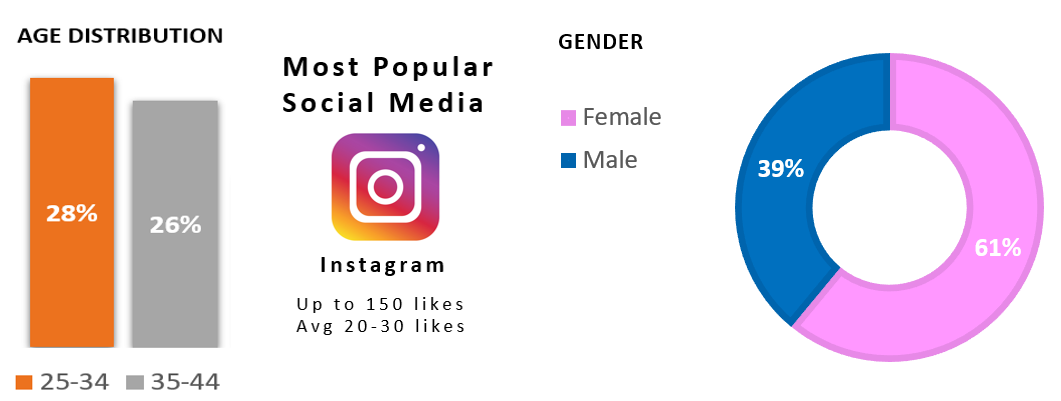
\includegraphics[width=0.8\linewidth,height=0.8\textheight]{/Users/leonardo.urbiola_fox/Desktop/R Studio/Audience/q4} \end{center}

\hypertarget{aditional-information}{%
\subsection{Aditional Information}\label{aditional-information}}

\hypertarget{education-level}{%
\subsubsection{\texorpdfstring{\href{https://www.census.gov/newsroom/press-releases/2022/educational-attainment.html\#:~:text=1\%20In\%202021\%2C\%2029.4\%25\%20of\%20men\%20age\%2025,more\%2C\%2053.1\%25\%20were\%20women\%20and\%2046.9\%25\%20were\%20men./}{Education
Level}}{Education Level}}\label{education-level}}

In 2021, the highest level of education of the population age 25 and
older in the United States was distributed as follows:

\begin{longtable}[]{@{}cc@{}}
\toprule()
\textbf{Total, 25 years and over} & \textbf{Percentage} \\
\midrule()
\endhead
Less than a high school diploma & 8.9 \% \\
High school graduates, no college & 27.9 \% \\
Some college or associate degree & 14.9 \% \\
Completed an Associate's degree & 10.5\% \\
Completed a Bachelor's degree & 23.5 \% \\
Advanced Degree & 14.4 \% \\
\bottomrule()
\end{longtable}

\hypertarget{spanish-language} of the total amount of leads come from \textbf{Texas}
  (\href{https://app.powerbi.com/groups/me/reports/f381dddc-6f32-4138-82a4-185b134a5c79/ReportSectionad6d6d8da06eb3248e83/}{IM
  Report})
\item
  In Texas \textbf{40.2\%} of the population are \textbf{Hispanic or
  Latino}
\item
  \textbf{85\%} of the 23.7 million people in Texas speak a language
  other than English. A large majority of those speak \textbf{Spanish}.
\end{itemize}

\begin{center}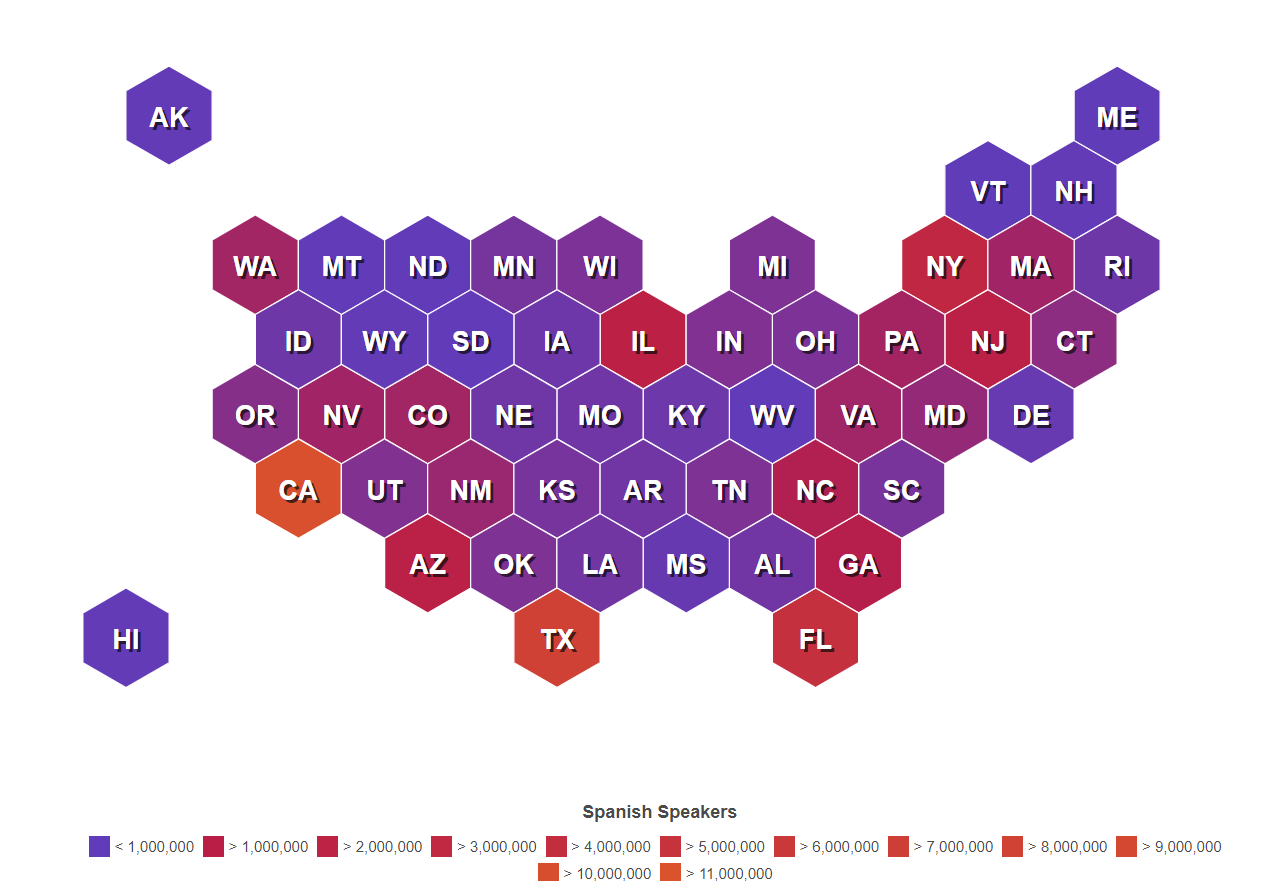
\includegraphics[width=0.9\linewidth,height=0.9\textheight]{/Users/leonardo.urbiola_fox/Desktop/R Studio/Audience/map1} \end{center}

\begin{center}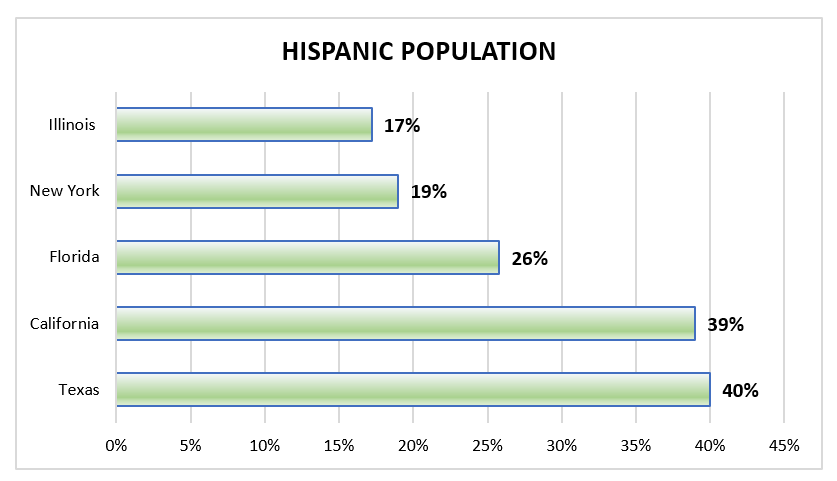
\includegraphics[width=0.9\linewidth,height=0.9\textheight]{/Users/leonardo.urbiola_fox/Desktop/R Studio/Audience/popu1} \end{center}

\hypertarget{employment-status}{%
\subsubsection{Employment Status}\label{employment-status}}

\begin{center}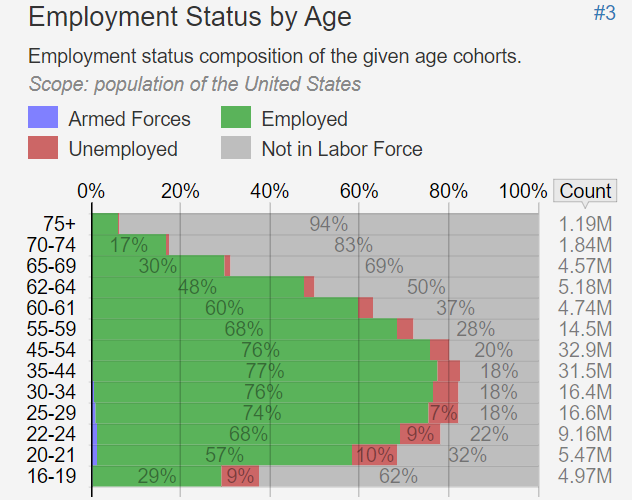
\includegraphics[width=0.8\linewidth,height=0.6\textheight]{/Users/leonardo.urbiola_fox/Desktop/R Studio/Audience/age_1} \end{center}

\begin{center}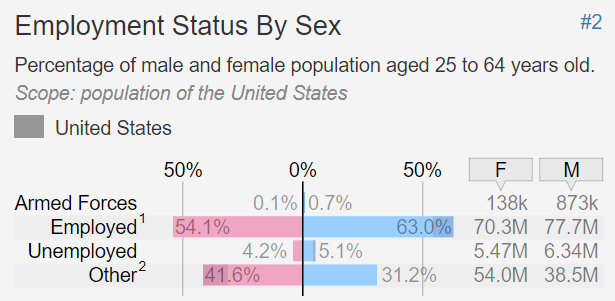
\includegraphics[width=0.75\linewidth,height=0.6\textheight]{/Users/leonardo.urbiola_fox/Desktop/R Studio/Audience/age_2} \end{center}

\hypertarget{recommendations}{%
\subsection{Recommendations}\label{recommendations}}

\hypertarget{age}{%
\subsubsection{Age}\label{age}}

Create content that is focused on audiences between \textbf{25 to 44
years old}. This age range provides more than 40\% of the people who
interact with Fox Pest Control.

\hypertarget{mobile-device}{%
\subsubsection{Mobile device}\label{mobile-device}}

Prioritize content for \textbf{mobile devices}. 64\% of our audience
interacts with our websites through mobile devices.

\hypertarget{gender}{%
\subsubsection{Gender}\label{gender}}

Although more than 60\% of our overall audience are \textbf{females} it
is recommended to create content for both genders because in most of the
branches the percent of females and males are relatively comparable.

\hypertarget{interest}{%
\subsubsection{Interest}\label{interest}}

The top 2 interests of the population who search for pest control are
\textbf{Home \& Garden/Home Decor} and \textbf{Real Estate/Residential
Properties}. The most popular reason is because most people want to
either protect or sell their homes. It is recommended to advertise Fox
Pest Control in real estate and home improvement retail websites.

\hypertarget{content-in-spanish}{%
\subsubsection{Content in Spanish}\label{content-in-spanish}}

Create Content in \textbf{Spanish}. 23\% of the leads received in 2022
come from Texas. 40\% of the population are Hispanic or Latino.
According to the U.S. Census in 2021, around 15\% of the population in
Texas did not speak English well and more than a third of the population
feel more comfortable speaking a language other than English.
Additionally, NY and IL are listed on the top 5 states where Spanish is
spoken. 45\% of the leads we obtained in 2022 are from these three
states.

\end{document}
